\section{Lagrangian equations for a single particle}
\label{ap:particles_eq}

As discussed in \ref{sec:Lagrangian} we now express the mass, momentum, and energy equation for a single Lagrangian particle. 

\subsection{Fundamental properties of a particle}

At this stage, we define some fundamental properties associated with each particle labeled $\alpha$.
Following the strategy of \citet{lhuillier2009rheology,lhuillier1992volume,zaepffel2011modelisation} and \citet[Chapter 2]{morel2015mathematical}
we define the mass $m_\alpha$, position of center of mass $\mathbf{x}_\alpha$, the momentum $\textbf{p}_\alpha$ and the total energy $E_\alpha$ of the particle $\alpha$, as
\begin{align}
    m_\alpha
    &= \intO{ \rho_d  }, 
    \\
    \textbf{x}_\alpha
    &= \frac{1}{m_\alpha }\intO{ \rho_d \textbf{x} }, 
    \\\textbf{p}_\alpha 
    &= \intO{ \rho_d \textbf{u}_d^0 },
    \label{eq:mass_pos}
    \\
    E_\alpha(t) 
    &=\frac{1}{m_\alpha} 
    \intO{ \rho_d [e_d^0 + (u_d^0)^2/2] }
    % \label{eq:momentum_energy}
\end{align}
% $\Omega_\alpha(t,\FF)$ is the time-dependent domain occupied by the particle $\alpha$ (see \ref{fig:Scheme}). 
% Subsequently, we define the velocity of the particle center of mass as
% \begin{equation*}
% \textbf{u}_\alpha = \frac{d \textbf{x}_\alpha}{dt}.
% \end{equation*}
% Replacing $\textbf{x}_\alpha$ by its definition (\ref{eq:mass_pos}) we obtain
% \begin{equation*}
%     \textbf{u}_\alpha = \frac{1}{m_\alpha}
%     \frac{d}{dt} 
%     \left(
%         \intO{ \rho_d \textbf{x} }
%     \right)
%     - \frac{1}{m_\alpha^2} \frac{d}{dt} \left(\intO{ \rho_d } \right)
%     \intO{ \rho_d \textbf{x} }.
% \end{equation*}
% %\tb{ A finaliser
% Using the Reynolds transport theorem (\ref{eq:reynolds_transport}) for both terms in parentheses and making use of the conservation of mass (\ref{eq:dt_rho}) and the definition of $\textbf{x}_\alpha(t,\FF)$ in the last term, gives
% \begin{equation}
%     \textbf{u}_\alpha = 
%     \frac{1}{m_\alpha}\intO{ \left[
%         \pddt (\textbf{x}\rho_d ) + \div\left(\textbf{u}_d^0 \textbf{x} \rho_d\right) 
%     \right]} \\
%     + \frac{1}{m_\alpha}\intS{ \textbf{x} \rho_d(\textbf{u}_\Gamma   - \textbf{u}_d^0) \cdot \textbf{n}_d }
%     -  \frac{\textbf{x}_\alpha}{m_\alpha}    \intS{ \rho_d(\textbf{u}_\Gamma   - \textbf{u}_d^0) \cdot \textbf{n}_d }
% \end{equation}
% Then by considering the mass conservation for the first term and noticing that $\grad \textbf{x} = \bm\delta$ with $\bm\delta$ the unit tensor, for the second term gives, 
% \begin{equation}
%     \textbf{u}_\alpha(t,\FF) = \frac{1}{m_\alpha(t,\FF)} \left(
%         \textbf{p}_\alpha(t,\FF)
%         +  \intS{\rho_d \textbf{r} (\textbf{u}_\Gamma^0 - \textbf{u}_d^0)\cdot \textbf{n}_d }
%         \right),
%         \label{eq:dt_y_alpha}
% \end{equation}
% where $\textbf{r}(\textbf{x},t) = \textbf{x} - \textbf{x}_\alpha(t)$. 
% In \ref{eq:dt_y_alpha}, it can be observed that the first component of the velocity represents the linear momentum divided by the mass of the particle. 
% This corresponds to the mass-averaged velocity over the volume of the particle.
% The second term in \ref{eq:dt_y_alpha} arises from the contribution of anisotropic mass transfer across the surface of the particle. 
% This mass transfer leads to the motion of the particle's center of mass, thereby contributing to the total velocity.
% To illustrate this concept, let us consider a fixed drop with no momentum lying over a very hot plate.
% In this scenario, we assume that the plate is sufficiently hot to induce evaporation, specifically on the bottom portion of the drop.
% Hence, under the effect of an anisotropic evaporation flux one may expect the second term to be non-negligible.
% Consequently, the center of mass of the drop has a non-zero velocity in the opposite direction of the plate, even though the momentum is assumed to be zero.
% Note that \ref{eq:dt_y_alpha} generalized usual expression of the center of mass velocity whom neglect the second term.
% In the following, for the sake of brevity we discard the dependency on $t$ and $\FF$ on the notations for all Lagrangian quantities denoted by the subscript $_\alpha$ and in particular $\Gamma_\alpha$ and $\Omega_\alpha$.
% Nevertheless, the reader must understand that all Lagrangian quantities and integration domains subscribed by $_\alpha$ are time and configuration-dependent. 

The particle's internal relative motions or the \textit{inner velocity} is given by $\textbf{w}_d^0 = \textbf{u}_d^0 - \textbf{u}_\alpha$. 
Substituting the inner velocity in the momentum definition (\ref{eq:mass_pos}) yields
\begin{equation}
    \label{eq:momentum_definition_1}
    \textbf{p}_\alpha
    = m_\alpha \textbf{u}_\alpha
    + \int_{\Omega_\alpha} \rho_d \textbf{w}_d^0 d\Omega.
\end{equation}
Alternatively, from \eqref{eq:dt_y_alpha}, we obtain
\begin{equation}
    \textbf{p}_\alpha
    =  m_\alpha \textbf{u}_\alpha
    - \int_{\Gamma_\alpha} \rho_d\textbf{r}(\textbf{u}_\Gamma^0 - \textbf{u}_d^0)\cdot \textbf{n}_d d\Sigma.
    \label{eq:momentum_definition}
\end{equation}
Therefore, the momentum of a particle can be seen as a sum of the mean velocity plus the integral of the fluctuations (\ref{eq:momentum_definition_1}), with the latter being equivalent to minus the first moment of mass transfer term (\ref{eq:momentum_definition}).
Indeed, by identification we obtain : $\intO{ \rho_d \textbf{w}_d^0 } = - \intS{  \rho_d\textbf{r} (\textbf{u}_\Gamma^0 - \textbf{u}_d^0)\cdot \textbf{n}_d }$. 
Hence, the internal velocity fluctuations within a fluid particle do not contribute to the total linear momentum $\textbf{p}_\alpha$, as long as the anisotropic mass transfer is negligible.  
In this study, we assume this to be the case, therefore, we can consider the classical relation $\textbf{p}_\alpha = m_\alpha \textbf{u}_\alpha$. 


Using the decomposition $\textbf{u}_d^0 = \textbf{u}_\alpha + \textbf{w}_d^0$, the total energy $E_\alpha$ can be decomposed according to
\begin{equation*}
    \label{eq:E_alpha_def}
    m_\alpha E_\alpha
    = m_\alpha e_\alpha 
    + W_\alpha
    + m_\alpha (u_\alpha)^2/2
    % + \gamma s_\alpha 
\end{equation*}
Consequently, the total energy of a particle is the contribution of :
its internal energy $m_\alpha e_\alpha = \intO{\rho_d^0 e_d^0}$; 
its internal kinetic energy, $W_\alpha =  \intO{\rho_d  (w_d^0)^2/2 }$;
its center of mass kinetic energy, $u_\alpha^2/2$. 
Finally, we introduce the total energy of both the volume and the surface of the particle, which is defined as 
\begin{equation*}
    m_\alpha E_\alpha^\text{tot}
    = 
    s_\alpha  E_{\alpha I}
    + m_\alpha E_\alpha
    = 
    s_\alpha \gamma 
    + m_\alpha E_\alpha
\end{equation*}
where we noted $s_\alpha = \intS{}$ the surface of the particle $\alpha$, meaning that $E_{\alpha I} s_\alpha = \gamma s_\alpha $ corresponds to the surface energy of the particle. 


In the objective of describing the shape as well as the deformation of a particle we now introduce the second moment of mass and first-order moment of momentum of a particle. 
Following \ref{eq:Q_n_definition} we define the second-order moment of mass and the first-order moment of momentum as 
\begin{equation}
    \textbf{M}_\alpha 
    = \intO{ \rho_d \textbf{r} \textbf{r} }
    \;\;\;\text{and}\;\;\;
    \textbf{P}_\alpha 
    = \intO{ \rho_d \textbf{r} \textbf{u}_d^0 },
    \label{eq:first_moment_of_momentum_def}
\end{equation}
respectively. 
Note that $\textbf{M}_\alpha$ is analogous to the inertia tensor $\textbf{I}_\alpha$ in solid mechanics, $\textbf{M}_\alpha$ and $\textbf{I}_\alpha$ are related through the expression $\textbf{I}_\alpha = (\bm\delta : \textbf{M}_\alpha)\bm\delta - \textbf{M}_\alpha$.
For a fluid with a constant density, the tensor $\textbf{M}_\alpha$ describes the second moment of the volume distribution around the particle center of mass.
Likewise, the tensor $\textbf{P}_\alpha$ describes the first moment of the velocity distribution within the particle volume. 
To provide a clearer physical interpretation of the moment of momentum tensor, we decompose $\textbf{P}_\alpha$ into two distinct parts, denoted as $\textbf{S}_\alpha$ and $\textbf{T}_\alpha$ such that,
$\textbf{P}_\alpha = \textbf{S}_\alpha+\textbf{T}_\alpha$, where $\textbf{S}_\alpha = \frac{1}{2}(\textbf{P}_\alpha + \textbf{P}_\alpha^\dagger)$ represents the symmetric part and $\textbf{T}_\alpha = \frac{1}{2}(\textbf{P}_\alpha - \textbf{P}_\alpha^\dagger)$ is the antisymmetric part of $\textbf{P}_\alpha$.
Then, the tensors $\textbf{S}_\alpha$ and $\textbf{T}_\alpha$ correspond respectively to the stretching and angular momentum of the particle $\alpha$. 
The tensor $\textbf{S}_\alpha$ quantifies how fast and in which direction the particle gets elongated or flattened, in other words it represents the mean rate of deformation experienced by the particle.
The tensor $\textbf{T}_\alpha$ is related to the angular momentum of the particle denoted by the pseudo vector $\bm\mu_\alpha = \intO{ \rho_d \textbf{r} \times \textbf{u}_d^0 }$. 
Indeed, both  $\textbf{T}_\alpha$ and $\bm{\mu}_\alpha$ represent the angular momentum and are related through $(\bm{\mu}_\alpha)_i = \epsilon_{ijk} (\textbf{T}_\alpha)_{jk} = \epsilon_{ijk} (\textbf{P}_\alpha)_{jk}$, where $\bm\epsilon$ is the third order alternating unit tensor or Levi-Cita tensor. 
Lastly, we also introduce the scalar $M_\alpha =\frac{1}{3}\bm\delta : \textbf{P}_\alpha = \frac{1}{3}\intO{ \rho_d \textbf{r} \cdot \textbf{u}_d^0 }.$, which quantifies the rate at which the particle is being compressed or expanded.
To better explain the implication of these quantities on the particle kinematics we provide in \ref{eq:scheme}, three plots representing possible inner velocity fields with their corresponding value of the moment of momentum tensor.
% Note that in \ref{eq:scheme} we explicit
\begin{figure}[h!]
    \centering
    \hfill
    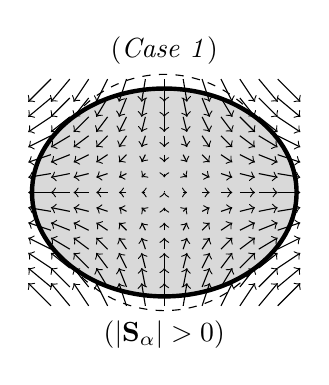
\begin{tikzpicture}[ultra thick,scale=0.6]
        \def\nRows{6}
        \def\nCols{6}
        \draw[dashed,thin] (0,0)circle(2.5);
        \draw[fill=gray!30] (0,0)ellipse(2.8 and 2.2);
        \foreach \x in {-\nRows,...,\nRows} {
            \foreach \y in {-\nCols,...,\nCols} {
                \pgfmathsetmacro\distance{veclen(\x*0.4, \y*0.4)};
                \pgfmathparse{\distance < 2.45 ? "blue" : "white"}
                \edef\colour{\pgfmathresult};
                \ifthenelse{\equal{\colour}{blue}}{                    
                    \draw[thin,->](\x*0.4,\y*0.4)--++(0.08*\x,-0.08*\y);
                }
            }
        }
        \node (txt) at (0,3){(\textit{Case 1})};
        \node (txt) at (0,-3){($|\textbf{S}_\alpha| > 0$)};
    \end{tikzpicture}
     \hfill
    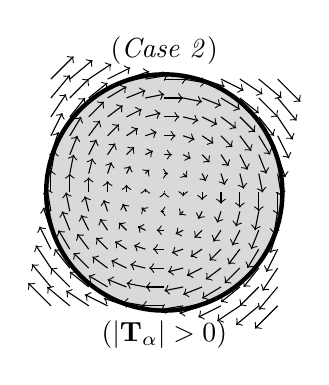
\begin{tikzpicture}[ultra thick,scale=0.6]
        \def\nRows{6}
        \def\nCols{6}
        \draw[fill=gray!30] (0,0)circle(2.5);
        \foreach \x in {-\nRows,...,\nRows} {
            \foreach \y in {-\nCols,...,\nCols} {
                \pgfmathsetmacro\distance{veclen(\x*0.4, \y*0.4)};
                \pgfmathparse{\distance < 2.5 ? "blue" : "white"}
                \edef\colour{\pgfmathresult};
                \ifthenelse{\equal{\colour}{blue}}{                    
                    \draw[thin,->](\x*0.4,\y*0.4)--++(0.08*\y,-0.08*\x);
                }
            }
        }
        \node (txt) at (0,3){(\textit{Case 2})};
        \node (txt) at (0,-3){($|\textbf{T}_\alpha| > 0$)};
    \end{tikzpicture}
    \hfill
    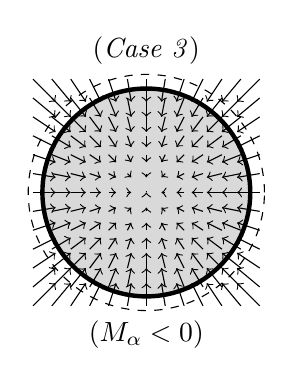
\begin{tikzpicture}[ultra thick,scale=0.6]
        \def\nRows{6}
        \def\nCols{6}
        \draw[dashed,thin] (0,0)circle(2.5);
        \draw[fill=gray!30] (0,0)circle(2.2);
        \foreach \x in {-\nRows,...,\nRows} {
            \foreach \y in {-\nCols,...,\nCols} {
                \pgfmathsetmacro\distance{veclen(\x*0.4, \y*0.4)};
                \pgfmathparse{\distance < 2.3 ? "blue" : "white"}
                \edef\colour{\pgfmathresult};
                \ifthenelse{\equal{\colour}{blue}}{                    
                    \draw[thin,->](\x*0.4,\y*0.4)--++(-0.08*\x,-0.08*\y);
                }
            }
        }
        \node (txt) at (0,3){(\textit{Case 3})};
        \node (txt) at (0,-3){($M_\alpha < 0$)};
    \end{tikzpicture}
    \hfill
    \caption{Graphical representation of the inner kinematics of an arbitrary particle under three scenarios. 
        The arrows represent the velocity field inside the particle, $\textbf{w}_d^0$, with the corresponding value of the moment of momentum tensor indicated below. 
        The operator $|\ldots|$ refers to the norm of the tensors. 
        According to the inner velocity field:
        (\textit{Case 1}) The particle experiences a mean rate of deformation, resulting in non-zero stretching of momentum along the principal axis of deformation;
        (\textit{Case 2}) The particle is rotating, leading to a non-zero angular momentum vector in the direction of rotation;
        (\textit{Case 3}) The particle undergoes compression, resulting in a negative trace of the moment of momentum.
    }
    \label{eq:scheme}
\end{figure}

% \section{Conservation laws}



% \subsection{Inside the volume}

 


% Let us consider the specific case of the momentum balance, i.e. $q_\alpha = \textbf{p}_\alpha$.
% In this situation, \ref{eq:dt_q_alpha} reads
% \begin{equation}
%     \ddt  \textbf{p}_\alpha
%     = \intO{ \rho_d\textbf{g} }
%     + \intS{ 
%         \left[
%         f_d^0 (\textbf{u}_\Gamma^0-\textbf{u}_d^0)
%          + \bm{\sigma}_d^0%\cdot\textbf{n}_d  
%         %+ \mathbf{\Phi}_d^0 
%         \right] 
%         \cdot \textbf{n}_d },
% \end{equation}
% first term reads as $\intO{ \rho_d\textbf{g} }$ 
% The first term on the right-hand side represents the total weight acting on the particle $\alpha$, 
% the second term represents the total source of momentum due to phase transfer, and it is expressed as, $\intS{ \rho_d \textbf{u}_d^0 (\textbf{u}_\Gamma^0-\textbf{u}_d^0)\cdot\textbf{n}_d }$,
% and the last term $\intS{ \bm{\sigma}_d^0\cdot\textbf{n}_d }$, represents the resultant of the hydrodynamic forces acting on the surface of the particle.
% It is important to note that under this form, the exchange terms are expressed as integrals of dispersed phase fields denoted by the subscript $_d$.
% Nevertheless, depending on the nature of the dispersed phase, these fields may not always be defined.
% For rigid particles the stress within the particle $\bm{\sigma}_d^0$ is indeterminate \citep{guazzelli2011}.  
% Hence, our objective is to express these exchange terms, in terms of the continuous phase field quantities instead of the dispersed phase fields, i.e. in terms of $\mathbf{\Phi}_f^0$ and $\textbf{u}_f^0$ rather than $\mathbf{\Phi}_d^0$ and $\textbf{u}_d^0$. 

%\subsection{On the interfaces}
 

%For completeness, we exposed in \ref{ap:particles_eq} a clear derivation of the mass, momentum and total energy equations for a single particle.
%The derivation takes place using the same hypothesis as it is exposed in \ref{ap:hypothesis}.
%Especially, it is shown that the integration of the kinetic energy jump condition corresponds to the Lagrangian derivative of the particle surface, see \ref{eq:int_u_I2}.
